\documentclass[a4paper,14pt]{extarticle}

% Путь до папки с общими шаблонами
\newcommand{\pathToCommonFolder}{/home/denilai/Documents/repos/latex/Common}
% Название работы в титуле
\newcommand{\workname}{Отчет по практическим работам 1-4}
% Название дисциплины в титуле
\newcommand{\discipline}{Технологические основы Инетернета вещей}
% Название кафедры в титуле
\newcommand{\kafedra}{Кафедра Математического обеспечения и стандартизации информационных технологий}
% Тема работы в титуле
\newcommand{\theme}{Знакомство с оборудованием}
% Должность преподавателя в титуле
\newcommand{\rang}{ассистент}

% ФИО студента в титуле
\newcommand{\studentfio}{К.~Ю.~Денисов}%\\Д.~Н.~Федосеев\\А.~М.~Сосунов}\\%К.~Ю.~Денисов\\%И.~А.~Кремнев
% ФИО преподавателя в титуле
\newcommand{\teacherfio}{Ю.~А.~Воронцов}


\usepackage{tabularx}


\usepackage{booktabs}
\newcolumntype{b}{X}
\newcolumntype{s}{>{\hsize=.5\hsize}X}
\newcommand{\heading}[1]{\multicolumn{1}{c}{#1}}

% установка размера шрифта для всего документа
%\fontsize{20pt}{18pt}\selectfont
\usepackage{extsizes} % Возможность сделать 14-й шрифт

% Вставка заготовки преамбулы
% Этот шаблон документа разработан в 2014 году
% Данилом Фёдоровых (danil@fedorovykh.ru) 
% для использования в курсе 
% <<Документы и презентации в \LaTeX>>, записанном НИУ ВШЭ
% для Coursera.org: http://coursera.org/course/latex .
% Исходная версия шаблона --- 
% https://www.writelatex.com/coursera/latex/5.3

% В этом документе преамбула

% Для корректного использования русских символов в формулах
% пакеты hyperref и настройки, связанные с ним, стоит загуржать
% перед загрузкой пакета mathtext



% поддержка русских букв
% кодировка шрифта
%\usepackage[T2A]{fontenc} 
\usepackage{pscyr}

% использование ненумеровонного абзаца с добавлением его в содержаниеl

\newcommand{\anonsection}[1]{\section*{#1}\addcontentsline{toc}{section}{#1}}
\newcommand{\sectionunderl}[1]{\section*{\underline{#1}}}


% настройка окружения enumerate
\usepackage{enumitem}
\setlist{noitemsep}
\setlist[enumerate]{labelsep=*, leftmargin=1.5pc}

\usepackage{hyperref}

% сначала ставить \usepackage{extsizes} % Возможность сделать 14-й шрифт
% для корректной установки полей вставлять преамбулу следует в последнюю очередь (но перед дерективой замены \rmdefault)
\usepackage[top=20mm,bottom=25mm,left=35mm,right=20mm]{geometry} % Простой способ задавать поля

\hypersetup{				% Гиперссылки
	unicode=true,           % русские буквы в раздела PDF
	pdftitle={Заголовок},   % Заголовок
	pdfauthor={Автор},      % Автор
	pdfsubject={Тема},      % Тема
	pdfcreator={Создатель}, % Создатель
	pdfproducer={Производитель}, % Производитель
	pdfkeywords={keyword1} {key2} {key3}, % Ключевые слова
	colorlinks=true,       	% false: ссылки в рамках; true: цветные ссылки
	linkcolor=red,          % внутренние ссылки
	citecolor=black,        % на библиографию
	filecolor=magenta,      % на файлы
	urlcolor=blue           % на URL
}

%%% Работа с русским языком
\usepackage{cmap}					% поиск в PDF
\usepackage{mathtext} 				% русские буквы в формулах
\usepackage[T2A]{fontenc}			% кодировка
\usepackage[utf8]{inputenc}			% кодировка исходного текста
\usepackage[english,russian]{babel}	% локализация и переносы
\usepackage{indentfirst}
\frenchspacing

%для изменения названия списка иллюстраций
\usepackage{tocloft}


\renewcommand{\epsilon}{\ensuremath{\varepsilon}}
\renewcommand{\phi}{\ensuremath{\varphi}}
\renewcommand{\kappa}{\ensuremath{\varkappa}}
\renewcommand{\le}{\ensuremath{\leqslant}}
\renewcommand{\leq}{\ensuremath{\leqslant}}
\renewcommand{\ge}{\ensuremath{\geqslant}}
\renewcommand{\geq}{\ensuremath{\geqslant}}
\renewcommand{\emptyset}{\varnothing}

% Изменения параметров списка иллюстраций
\renewcommand{\cftfigfont}{Рисунок } % добавляем везде "Рисунок" перед номером
\addto\captionsrussian{\renewcommand\listfigurename{Список иллюстративного материала}}

\newcommand{\tm}{\texttrademark\ }
\newcommand{\reg}{\textregistered\ }


%%% Дополнительная работа с математикой
\usepackage{amsmath,amsfonts,amssymb,amsthm,mathtools} % AMS
\usepackage{icomma} % "Умная" запятая: $0,2$ --- число, $0, 2$ --- перечисление

%% Номера формул
%\mathtoolsset{showonlyrefs=true} % Показывать номера только у тех формул, на которые есть \eqref{} в тексте.
%\usepackage{leqno} % Нумереация формул слева

%% Свои команды
\DeclareMathOperator{\sgn}{\mathop{sgn}}

%% Перенос знаков в формулах (по Львовскому)
\newcommand*{\hm}[1]{#1\nobreak\discretionary{}
{\hbox{$\mathsurround=0pt #1$}}{}}


% отступ для первого абзаца главы или параграфа
%\usepackage{indentfirst}

%%% Работа с картинками
\usepackage{graphicx}  % Для вставки рисунков
\graphicspath{{images/}{screnshots/}}  % папки с картинками
\DeclareGraphicsExtensions{.pdf,.png,.jpg}
\setlength\fboxsep{3pt} % Отступ рамки \fbox{} от рисунка
\setlength\fboxrule{1pt} % Толщина линий рамки \fbox{}
\usepackage{wrapfig} % Обтекание рисунков текстом

%%% Работа с таблицами
\usepackage{array,tabularx,tabulary,booktabs} % Дополнительная работа с таблицами
\usepackage{longtable}  % Длинные таблицы
\usepackage{multirow} % Слияние строк в таблице

%%% Теоремы
\theoremstyle{plain} % Это стиль по умолчанию, его можно не переопределять.
\newtheorem{theorem}{Теорема}[section]
\newtheorem{proposition}[theorem]{Утверждение}

\theoremstyle{plain} % Это стиль по умолчанию, его можно не переопределять.
\newtheorem{work}{Практическая работа}[part]


 
 
\theoremstyle{definition} % "Определение"
\newtheorem{corollary}{Следствие}[theorem]
\newtheorem{problem}{Задача}[section]
 
\theoremstyle{remark} % "Примечание"
\newtheorem*{nonum}{Решение}



%%% Программирование
\usepackage{etoolbox} % логические операторы

%%% Страница

%	\usepackage{fancyhdr} % Колонтитулы
% 	\pagestyle{fancy}
%   \renewcommand{\headrulewidth}{0pt}  % Толщина линейки, отчеркивающей верхний колонтитул
% 	\lfoot{Нижний левый}
% 	\rfoot{Нижний правый}
% 	\rhead{Верхний правый}
% 	\chead{Верхний в центре}
% 	\lhead{Верхний левый}
%	\cfoot{Нижний в центре} % По умолчанию здесь номер страницы

\usepackage{setspace} % Интерлиньяж
\onehalfspacing % Интерлиньяж 1.5
%\doublespacing % Интерлиньяж 2
%\singlespacing % Интерлиньяж 1

\usepackage{lastpage} % Узнать, сколько всего страниц в документе.

\usepackage{soul} % Модификаторы начертания


\usepackage[usenames,dvipsnames,svgnames,table,rgb]{xcolor}


\usepackage{csquotes} % Еще инструменты для ссылок

%\usepackage[style=authoryear,maxcitenames=2,backend=biber,sorting=nty]{biblatex}

\usepackage{multicol} % Несколько колонок

\usepackage{tikz} % Работа с графикой
\usepackage{pgfplots}
\usepackage{pgfplotstable}

% модуль для вставки рыбы
\usepackage{blindtext}

\usepackage{listings}
\usepackage{color}


% для поворота отдельной страницы. Использовать окружение \landscape
\usepackage{pdflscape} 
\usepackage{rotating} 


\definecolor{mygreen}{rgb}{0,0.6,0}
\definecolor{mygray}{rgb}{0.5,0.5,0.5}
\definecolor{mymauve}{rgb}{0.58,0,0.82}


% пример импорта файла
%\lstinputlisting{/home/denilai/repomy/conf/distributions}

\lstset{
	language=Python,
	basicstyle=\footnotesize,        % the size of the fonts that are used for the code
	numbers=left,                    % where to put the line-numbers; possible values are (none, left, right)
	numbersep=5pt,                   % how far the line-numbers are from the code
	numberstyle=\tiny\color{mygray}, % the style that is used for the line-numbers
	stepnumber=2,                    % the step between two line-numbers. If it's 1, each line will be numbered
	% Tab - 2 пробела
	tabsize=2,    
	% Автоматический перенос строк
	breaklines=true,
	frame=single,
	breakatwhitespace=true,
	title=\lstname 
}



\author{Кирилл Денисов}
\title{Лабораторная работа №1}
\date{\today}

\renewcommand{\withouttheme}{1}

%если нужна тема работы в отчете, то указать в скобках что-либо, иначе оаставить пустым
%\renewcommand{\withouttheme}{}
%если нужна дата представления отчета, то указать в скобках что-либо
%\renewcommand{\withoutsubmissiondate}{1}

% установка полуторного интервала
% \usepackage{setspace}  
% \onehalfspacing

% использовать Times New Roman
\renewcommand{\rmdefault}{ftm}


\begin{document}
	\thispagestyle{empty}
	% Вставка первого титульного листа
	% Есть две версии титульного листа - одиночный (titul) и групповой (titulAll)
	%\newcommand{\withouttheme}{} добавить эту переменную для определения, нужна ли тема
%     {} - нужна
%    {1} - не нужна

%\newcommand{\withoutsubmissiondate}{} добавить эту переменную для определения, нужен ли срок предоставления отчета
%     {} - нужен
%    {1} - не нужен

\renewcommand{\studentfio}{К.~Ю.~Денисов\\
			%	& & \hfill И.~А.~Кремнев \\
				& & \hfill А.~М.~Сосунов\\
				& & \hfill Д.~Н.~Федосеев}

\begin{center}
	\begin{figure}[h!]
		\begin{center}
			%\vspace{10ex}
			
\includegraphics[width=0.17\linewidth]{\pathToCommonFolder/gerb}
			%\caption{}\label{pic:first}
			%	\vspace{5ex}
		\end{center}	
	\end{figure}
	\small	МИНОБРНАУКИ РОССИИ \\
	Федеральное государственное бюджетное образовательное учреждение\\
	высшего образования\\
	\normalsize					
	\textbf{«МИРЭА – Российский технологический университет»\\
		РТУ МИРЭА}\\
	\noindent\rule{1\linewidth}{1pt}\\
	Институт информационных технологий\\ %\vspace{2ex}
	\kafedra\\
	\vspace{3ex}
	\large \textbf{\workname}  \\
	%\vspace{1ex}
	по дисциплине\\ «\discipline» \\
	\vspace{3ex}
	\if \withouttheme
	\textbf{Тема работы:}\\ <<\theme>>
	\fi
	\vspace{6ex}
	\small
	\begin{table}[h!]
		\begin{tabular}{lp{0.6\linewidth}l}
			\textbf{Выполнили:} & студенты группы ИВБО-02-19 & \\ 
			& & \hfill \studentfio \\%Д.~Н.~Федосеев\\%А.~М.~Сосунов\\%К.~Ю.~Денисов\\%И.~А.~Кремнев
			\textbf{Принял:} & \rang & \\
			& & \hfill \teacherfio\\
		\end{tabular}
	\end{table}

	\normalsize
	
	\vfill
	Москва 2021
	
\end{center}
	\newpage
	\tableofcontents
	\newpage
	%\listoftables
	

\section{Практическая работа №1.\\Знакомство с оборудованием}

\subsection {Устройство стенда}
Работа на практических занятиях проводится с использованием стенда (чемодана\textbf{ WBdemo-kit v.2}), содержащего типовой набор оборудования в <<умном доме>>.

Стенд состоит из компонентов, расположение которых можно увидеть на Рис. \ref{fig:wb-demo-kit1}-\ref{fig:wb-demo-kit2}. В таблице \ref{tab:device-list} приводится их полный список.
 
% TODO: \usepackage{graphicx} required
\begin{figure}[htpb]
	\centering
	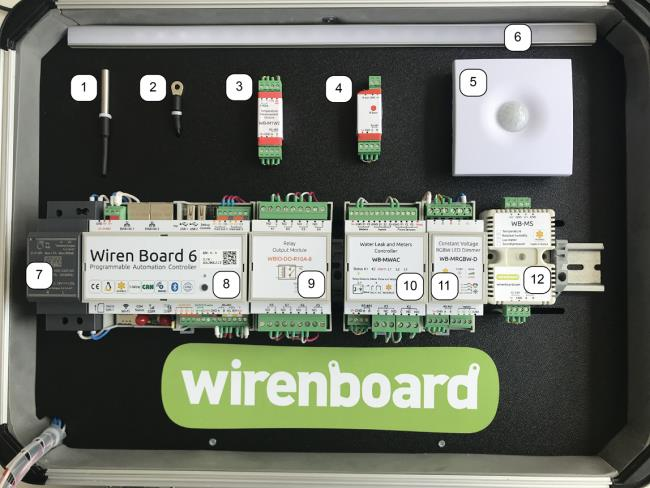
\includegraphics[width=0.6\linewidth]{images/wb-demo-kit1}
	\caption{Компоненты, расположенные на верхней крышке WB-demo-kit}
	\label{fig:wb-demo-kit1}
\end{figure}
 
 % TODO: \usepackage{graphicx} required
 \begin{figure}[htpb]
 	\centering
 	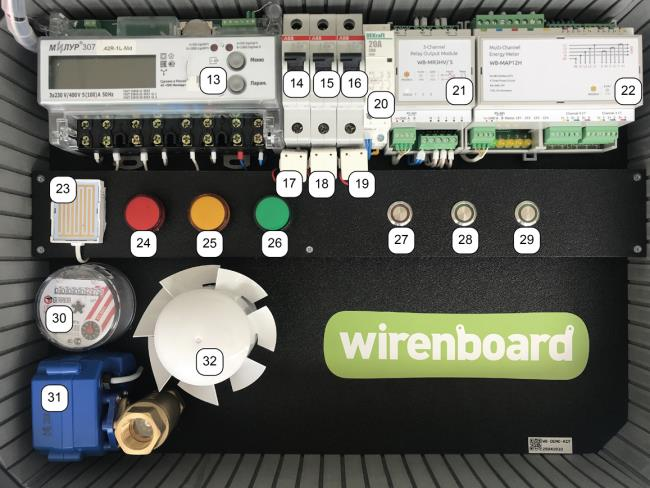
\includegraphics[width=0.6\linewidth]{images/wb-demo-kit2}
 	\caption{Компоненты, расположенные на нижней крышке WB-demo-kit}
 	\label{fig:wb-demo-kit2}
 \end{figure}

\begin{center}
	\begin{table}[htbp]
	%\small
	\begin{tabular}{|r|p{0.8\linewidth}|}
		\hline
		\multicolumn{1}{|c|}{\textbf{Номер}} & \multicolumn{1}{c|}{\textbf{Название}} \\ \hline\hline
		1 & Датчик температуры 1-wire DS18B20 \\ \hline
		2 & Датчик температуры 1-wire DS18B20 \\ \hline
		3 & Преобразователь 1-Wire — Modbus RTU WB-M1W2 \\ \hline
		4 & Устройство ИК-управления WB-MIR \\ \hline
		5 & Настенный комбинированный датчик WB-MSW v.3 \\ \hline
		6 & RGB лента в профиле \\ \hline
		7 & Блок питания HDR-30-24 \\ \hline
		8 & Контроллер Wiren Board 6 с модулем резервного питания для Wiren Board 6 WBMZ2-BATTERY \\ \hline
		9 & Модуль ввода-вывода WBIO-DO-R10A-8 \\ \hline
		10 & Модуль обнаружения протечек WB-MWAC \\ \hline
		11 & Диммер светодиодных лент на DIN-рейку WB-MRGBW-D \\ \hline
		12 & Комбинированный датчик WB-MS \\ \hline
		13 & Электросчетчик "Милур 307" \\ \hline
		14 & Автомат питания набора (L1) \\ \hline
		15 & Автомат питания вентилятора (L2) \\ \hline
		16 & Автомат питания контактора (L3) \\ \hline
		17 & Трансформатор тока 25 А (L1) \\ \hline
		18 & Трансформатор тока 25 А (L2) \\ \hline
		19 & Трансформатор тока 25 А (L3) \\ \hline
		20 & Контактор 220 В \\ \hline
		21 & Модуль реле 3-канальный WB-MR3 \\ \hline
		22 & Многоканальный измеритель WB-MAP12H \\ \hline
		23 & Датчик протечки \\ \hline
		24 & Индикатор 1 (протечка) \\ \hline
		25 & Индикатор 2 (вентилятор) \\ \hline
		26 & Индикатор 3 (контактор) \\ \hline
		27 & Кнопка 1 (подача воды, сброс аварии по протечке) \\ \hline
		28 & Кнопка 2 (вентилятор) \\ \hline
		29 & Кнопка 3 (контактор) \\ \hline
		30 & Импульсный счетчик расхода воды с имитацией потока \\ \hline
		31 & Шаровой кран с электроприводом \\ \hline
		32 & Вентилятор \\ \hline
	\end{tabular}
    \caption{Список компонентов демонстрационного набора WB-demo-kit}
	\label{tab:device-list}
\end{table}
\end{center}

	
\subsection{Ход работы}
В ходе выполнения данной практической работы были изучены и отработаны на практике следующие категории преднастроенного функционала (сценарии) стенда \textbf{Wb-demo-kit v.2}:
\begin{enumerate}
	\item Энергопотребление и контроль питания;
	\item Управление внешними силовыми устройствами;
	\item Мониторинг качества воздуха и управление вентиляцией;
	\item Мониторинг водоснабжения и протечек.
\end{enumerate}
Опишем порядок действий, производимых в рамках отработки предложенных сценариев:
\paragraph*{Включение стенда}
Убедившись, что стенд подключен к электросети, включим автоматы в порядке слева-направо, т.е. 14, 15, 16.
Включим контроллер (8), нажав на кнопку на корпусе. Когда индикатор контроллера
начнет мигать зеленым светом, контроллер будет готов к работе.
\paragraph*{Работа с функционалом контроля электропитания}
%\begin{enumerate}
	\script \textbf{Проверка наличия сетевого напряжения}
	
	Выключим автомат (14). Через несколько секунд индикатор контроллера (8) несколько раз
	часто моргнет красным и раздастся предупреждающий звуковой сигнал. Это означает, что
	сетевое напряжение отсутствует. Часть модулей продолжит питаться от встроенного в
	контроллер аккумуляторного модуля. Синий индикатор на блоке питания (7) погаснет
	примерно через 30 секунд.
	
	% TODO: \usepackage{graphicx} required
	\begin{figure}[htbp]
		\centering
		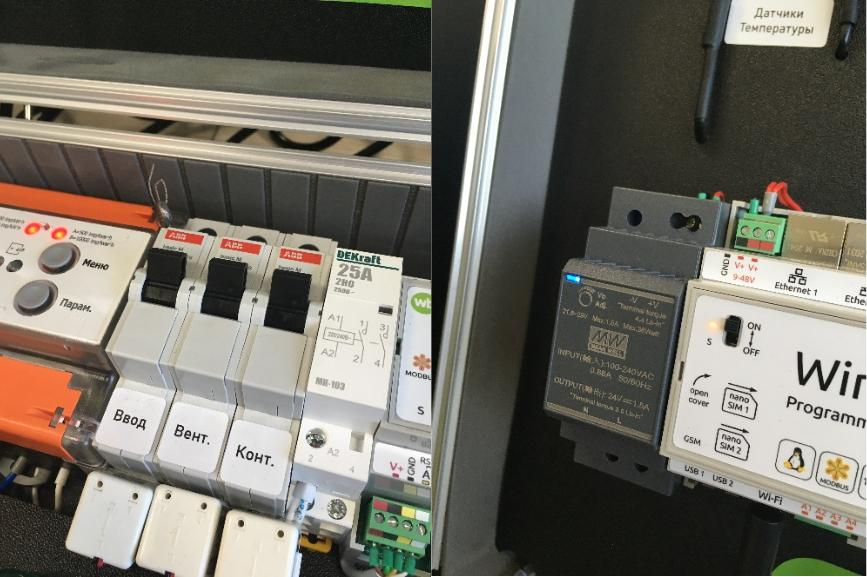
\includegraphics[width=0.6\linewidth]{images/1}
		\caption{Наличие сетевого напряжения}
		\label{fig:1}
	\end{figure}
	\script \textbf{Контроль повышенного энергопотребления}
	
	Включим вентилятор кнопкой (28). Загорится зеленая подсветка кнопки. Через некоторое
	время загорится желтый индикатор (25) --- это означает, что счетчик (22) детектирует
	энергопотребление на фазе, к которой подключен вентилятор. Не касаясь лопастей
	вентилятора, остановим его. Через несколько секунд счетчик (22) определит повышенное
	энергопотребление застопоренного вентилятора и контроллер отключит его. Погаснет
	зеленая подсветка кнопки (28), а затем -- желтый индикатор (25).	

% TODO: \usepackage{graphicx} required
\begin{figure}[htbp]
	\centering
	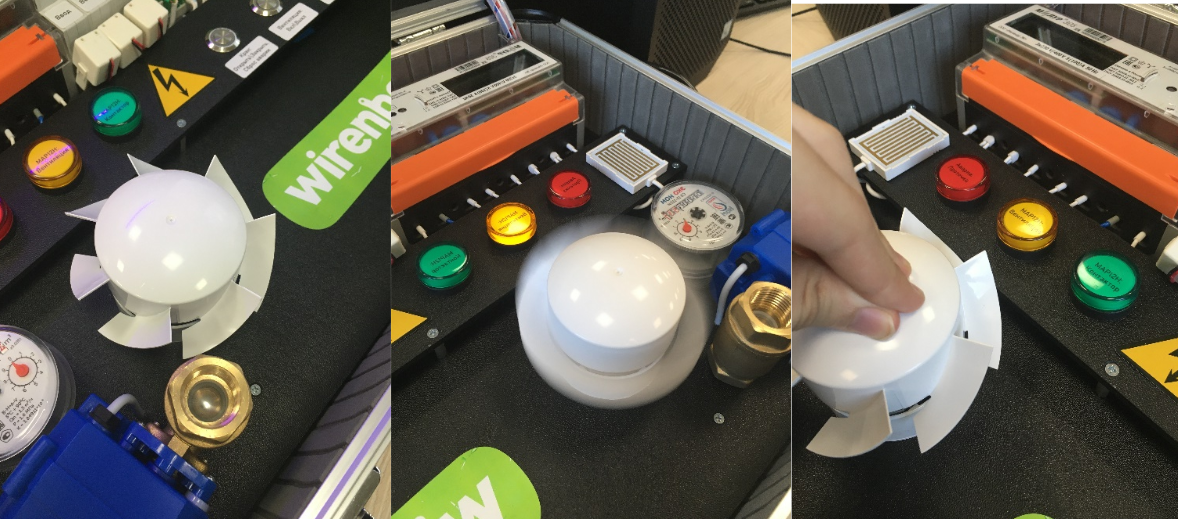
\includegraphics[width=0.6\linewidth]{images/fan}
	\caption{Контроль повышенного энергопотребления}
	\label{fig:fan}
\end{figure}

	
	\script  \textbf{Контроль автоматов}
	
	Отключим автоматы (15) и (16). Через несколько секунд начнет мигать подсветка кнопок
	(28) и (29), что означает, что напряжение на выходах автоматов пропало. Включим
	автоматы снова -- подсветка кнопок перестанет мигать.	
	
	% TODO: \usepackage{graphicx} required
	\begin{figure}[htbp]
		\centering
		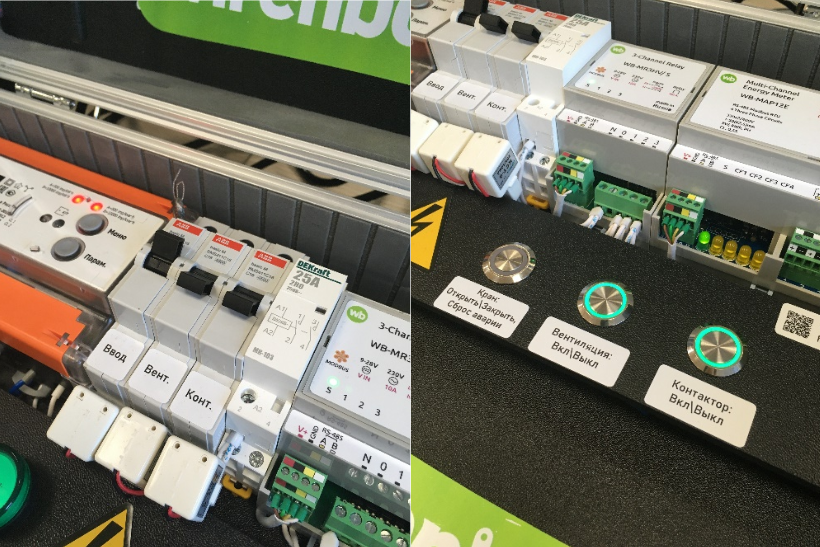
\includegraphics[width=0.6\linewidth]{images/power-off}
		\caption{Контроль автоматов}
		\label{fig:power-off}
	\end{figure}
	
%\end{enumerate}
\paragraph* {Управление внешними силовыми устройствами}
	\script \textbf{Управление контактором}

	Нажмем кнопку (29). Подсветка кнопки загорится зеленым, при этом сработает
	контактор (20). Через некоторое время загорится индикатор (26), что означает обнаружение
	энергопотребления на соответствующей фазе счетчиком (22). Нажмем кнопку (29) --
	контактор выключится, подсветка кнопки погаснет, а через несколько секунд погаснет и
	индикатор энергопотребления (26).
\paragraph*{Мониторинг качества воздуха}
	\script \textbf{Определение уровня $CO_2$} 
	
	При допустимом уровне концентрации $CO_2$ в помещении индикатор датчика (5)
	мигает зеленым светом. Если несколько раз на него энергично подуть, то через 15-20 секунд
	индикатор начнет мигать красным, что свидетельствует о превышении концентрации $CO_2$.
	При достижении нормальной концентрации датчик снова будет мигать зеленым.
\paragraph*{Мониторинг водоснабжения и протечек}
	\script \textbf{Работа модуля защиты от протечек}
	
	Нажмем кнопку (27). Откроется шаровой кран (31), а счетчик (30) начнет вращаться,
	имитируя поток воды в системе водоснабжения. Прикоснемся с небольшим усилием
	слегка влажным пальцем или смоченной салфеткой к датчику протечки.
	
	Шаровой кран перекроет поток воды, счетчик перестанет
	вращаться, загорится красный индикатор протечки (24), подсветка кнопки (27) начнет
	мигать, а модуль обнаружения протечек (10) будет выдавать непрерывный звуковой сигнал
	(на самом модуле будет гореть индикатор \textit{Alarm}). Для сброса аварийной ситуации
	(<<Протечка устранена>>) снова нажмем кнопу (27).
	Кнопкой 27 можно открывать и закрывать шаровой кран с электроприводом,
	последовательно нажимая на нее.
	
	% TODO: \usepackage{graphicx} required
	\begin{figure}[htbp]
		\centering
		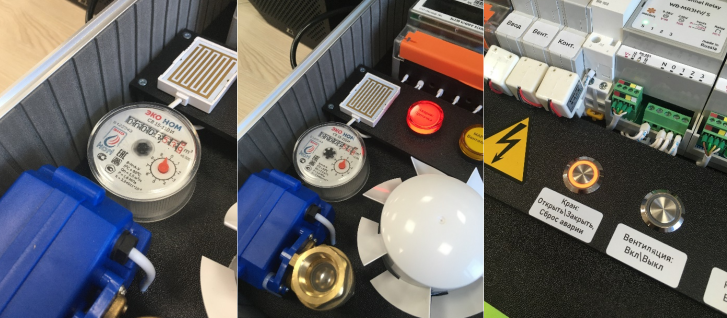
\includegraphics[width=0.6\linewidth]{images/waterproof}
		\caption{Мониторинг водоснабжения и протечек}
		\label{fig:waterproof}
	\end{figure}
	
\paragraph*{Выключение стенда}
	Для выключения оборудования сначала выключим контроллер (8), после -- автоматы в
	порядке справа-налево (т.е. 16, 15, 14).
	
\anonsubsection{Вывод}
В ходе данной практической работы мы познакомились с демонстрационным стендом\textbf{ WB-demo-kit v.2}, изучили и отработали на практике основные сценарии взаимодействия с входящими в его состав компонентами.

\newpage

\section{Дополнительные задания к работе №1}
\subsection{Сценарии применения технологий IoT}
Интернет вещей (Internet of Things, IoT) --- это множество физических объектов, подключенных к интернету и обменивающихся данными. Концепция IoT может существенно улучшить многие сферы нашей жизни и помочь нам в создании более удобного, умного и безопасного мира. Примеры Интернета вещей варьируются от носимых вещей, таких как умные часы, до умного дома, который умеет, например, контролировать и автоматически менять степень освещения и отопления. 
\subsubsection*{Умный дом}

Умный дом --- совокупность автоматизированного пространства и <<умных>> вещей и приборов в доме, связанных вместе одной сетью.

Умные дома появились намного раньше Интернета вещей -- например, в 1985 году в США была система \textit{Unity} — она управляла безопасностью дома.

Однако современный умный дом подразумевает под собой не только управление безопасностью — в него могут быть включены и другие системы.
\subsubsection*{Умное освещение}
Проект умного дома может предусматривать различные сценарии освещения:
\begin{itemize}
	\item Схема умного дома со сценарием <<Перед сном>> предполагает установку прикроватных ламп на комфортном для чтения уровне.
	\item Одно нажатие кнопки <<Все выключено>> гасит свет во всем доме.
	\item Сценарий <<Обнаружение движения>> предполагает включение света на заданную мощность при обнаружении датчиком движения в зоне его действия.
\end{itemize}

\subsubsection*{Умная музыка}
Здесь интересны следующие сценарии Умного дома:
\begin{itemize}
	\item Трансляция сохраненной музыке по всему дому через распределенные звуковые зоны, доступ к которым осуществляется через  смартфон и сенсорные экраны.
	\item Автоматическое включение музыки в ванной при включении света в душе.
	\item Установка сенсорного экрана за водонепроницаемым настенным креплением в душе для управления музыкой. 
\end{itemize}
\subsubsection*{Развлекательная автоматизация}
Пример развлекательных сценариев
\begin{itemize}
	\item  Одно нажатие кнопки с подсветкой запускает сценарий «Вечеринка», предусматривающий освещение ключевых декоративных элементов с возможностью настраивания списка воспроизведения, запускаемого автоматически.
	\item Возможность получать уведомления о прибытии гостей путем передачи звукового сигнала через динамики аудиозоны.
\end{itemize}
\subsubsection*{Умная безопасность}
\begin{itemize}
	\item Встроенные оповещения, уведомляющие о том, что входная дверь оставлена открытой более пяти минут или если парадные ворота приоткрыты более чем на десять минут.
	\item  Доступ к видеопотоку системы безопасности удаленно со своего смартфона из любой точки мира.
	\item Получение уведомлений об обнаружении движения камерами видеонаблюдения.
	\item Возможность создания сценария на случай нарушения безопасности. Скажем, при получении определенного сигнала Умный дом включает освещение на 100\%, автоматически закрывает входную дверь, открывает моторизованные шторы, и передает на каждый телевизор сигнал со всех камер наблюдения.
	\item Создание временных кодов доступа гостям, если они посетят дом в отсутствие хозяев. Те будут получать уведомление о каждом таком визите.
\end{itemize}
\subsubsection*{Система климат-контроля}
\begin{itemize}
	\item Программирование штор на автоматическое открывание и закрывание в зависимости от положения солнца и загруженности дома.
	\item Программирование на <<Пробуждение>> --- постепенное открывание штор с постепенным увеличением освещения в течении пяти минут и установки температуры на желаемый уровень.
	\item Розжиг камина с помощью смартфона или планшета из любой точки дома.
\end{itemize}

\subsubsection*{Экономичные идеи автоматизации}
\begin{itemize}
	\item Измерять энергопотребление всего дома, схема за схемой, автоматически с помощью системы домашней автоматизации.
	\item Автоматизировать освещение в доме таким образом, чтобы обеспечить максимальное энергосбережение.
	\item Настроить опрыскиватели и газонные системы на автоматическое реагирование на погодные условия (чтобы исключить, полив газона в дождливые дни).
\end{itemize}
\subsubsection*{Идеи для голосового управления}
\begin{itemize}
	\item  <<Окей, Google, доброе утро>>. Этот сценарий предусматривает мягкое включение света в спальне, а затем на кухне и одновременный запуск плейлиста.
	\item <<Алиса, включи время вечеринки>>. Программа опускает диско-шар с потолка, включает светодиодные индикаторы, меняющие цвет, включает любимый плейлист для вечеринок на максимальную громкость.
	\item <<Поставь фильм в очередь>>. Голосовая команда запускает проигрыватель \textit{Blu-ray}, приглушает свет до 30\%, рисует тени и устанавливает идеальную атмосферу для кино-сеанса.
	\item  <<Окей, включи Режим сна>>. Сценарий предусматривает закрытие штор, запирание дверей и запуск расслабляющего плейлиста за час до отхода ко сну.
	\item  <<Окей, Google, пора идти>>. Программа мигает светом в детских, издает раздражающий звук туманного рожка и дает понять, что пора обуваться и выходить из дома.
	\item 
\end{itemize}


То есть по сути умный дом является посредником между пользователем и умными приборами --- он объединяет все их показания и выводит их пользователю в удобном для него виде --- на экран телевизора или смартфона, или же в устной форме. Ну и разумеется умный дом обрабатывает все команды пользователя и передает их приборам --- к примеру вы едете домой жарким летом и вам хочется прохлады в доме: достаточно отдать команду умному дому со смартфона и тот включит кондиционер.
\subsection {Стандарты и технологии передачи IoT}

Сегодня в решениях для домашней автоматизации (Home Automation) наблюдается настоящая война стандартов. Отдать предпочтение какому-либо достаточно сложно, поскольку у каждого из них есть свои сильные и слабые стороны.
\subsubsection*{Wi-Fi}
Wi-Fi может казаться самым очевидным решением для домашней автоматизации. Такую точку зрения поддерживает, прежде всего, его широкое распространение – по утверждениям консорциума Wi-Fi Alliance уже сегодня более 50% интернет-трафика приходится именно на долю Wi-Fi.
\subsubsection*{BlueTooth}
Исходный стандарт BlueTooth известен еще с 1994 г. Технология, изначально ориентированная на обмен данными между мобильными телефонами, сегодня стала одной из основных для связи между узлами и подключения периферийных устройств в локальных сетях. Однако даже после этого стандарт никак не подходил для организации сетей home automation.

Ситуация изменилась с появлением в 2010 г. BlueTooth Low Energy. Она разрабатывалась с прицелом на работу с компактными автономными устройствами, для многих из которых источниками служат малогабаритные маломощные батарейки.

Такое решение одной из основных проблем домашней автоматизации не могло не привлечь внимание разработчиков. Однако потенциал технологии до сих пор не получил реальной оценки, перспективы ее применения так и остаются неясными.
\subsubsection*{Z-Wave}
Z-Wave – стандарт, разработанный в 1999 г. специально для получения сигналов датчиков и управления исполнительными устройствами «умного дома». Основное его отличие – работа с миниатюрными девайсами с низким энергопотреблением. Используется радиочастотный диапазон 800-900 Мгц (нелицензируемый), в котором скорость передачи составляет до 100 кбит/с (для устройств спецификации Z-Wave Plus). Основная топология – mesh-сеть с маршрутизацией «от источника».
\subsubsection*{ZigBee}
Стандарт ZigBee, как и Z-Wave ориентирован на работу с маломощными компактными устройствами home automation и на сегодня, пожалуй, единственный кто может составить ему достойную конкуренцию и даже выигрывать в этой борьбе.

В отличие от Z-Wave использует стандартный нелицензируемый диапазон частот 2.4 ГГц. Отличаются и требования к сертификации. У подхода есть собственные преимущества и недостатки.
\subsubsection*{Подводя итог}
Рассматривая достоинства и недостатки различных технологий для «умного дома», можно сделать выводы:
\begin{itemize}
	\item От технологии Wi-Fi лучше отказаться. Использовать ее рационально только в том случае, когда необходимо передавать данные сенсоров в облачное хранилище или некоторым устройствам необходим выход в интернет (например, «умному» холодильнику – для заказа продуктов в магазине).
	\item BlueTooth LE можно рассматривать как перспективную технологию, однако придется дождаться появления на рынке нужного ассортимента девайсов (датчиков и исполнительных устройств).
	\item Использование Z-Wave – хорошее решение, однако при его применении придется внимательно отнестись к подбору устройств по рабочим частотам и быть готовым к значительным расходам на систему.
	\item ZigBee – отличный вариант с точки зрения масштабов и стоимости, однако обязательным условием работоспособности системы становится проверка совместимости ее компонентов.
\end{itemize}

\if
В связи с быстрым развитием Интернета вещей и исключительными особенностями данной сети (например, устройства с низким энергопотреблением, низкие скорости передачи и т.д.) возникла необходимость в создании протоколов, которые будут удовлетворять данным требованиям. 

В общем случае протоколы делят на группы в зависимости от участка сети, на котором они используются. Так в рамках концепции Интернета вещей существуют следующие участки: сенсорный узел --- сенсорный узел (самый распространенный протокол DDS), сенсорный узел --- сервер (CoAP, MQTT, XMPP, STOMP), сервер --- сервер (AMQP). Существует множество протоколов передачи данных, в качестве примера приведены самые популярные.
\begin{itemize}
	\item DDS \textit{(Data Distribution Service)} --- реализует шаблон публикации-подписки для отправки и приема данных, событий и команд среди конечных узлов. Узлы-издатели создают информацию, <<topic>> (темы, разделы: температура, местоположение, давление) и публикуют шаблоны. Узлам, заинтересовавшимся в данных разделах, DDS прозрачно доставляет созданные шаблоны. В качестве транспорта --- UDP. Также DDS позволяет управлять параметрами QoS (качество облуживания).
	
	\item CoAP \textit{(Constrained Application Protocol)} --- с точки зрения пользователя похож на протокол HTTP, но отличается малым размером заголовков, что подходит для сетей с ограниченными возможностями. Использует архитектуру клиент-сервер и подходит для передачи информации о состоянии узла на сервер (сообщения GET, PUT, HEAD, POST, DELETE, CONNECT). В качестве транспорта --- UDP.
	
	\item XMPP \textit{(Extensible Messaging and Presence Protocol)} --- давно используется в сети Интернет для передачи сообщений в режиме реального времени, благодаря формату XML подходит для использования в сетях IoT. Работает поверх архитектур издатель-подписчик и клиент-сервер. Также используется для адресации устройств в небольших сетях (адресация вида <<name@domain.com>>).
	
	\item MQTT \textit{(Message Queue Telemetry Transport)} --- осуществляет сбор данных от множества узлов и передачу на сервер. Основывается на модели издатель-подписчик с использованием промежуточного сервера --- брокера (приоритезация сообщений, формирование очередей и др.). В качестве транспорта --- TCP. На основе MQTT был сформирован специализированный протокол MQTT-SN для сенсорных сетей.
\end{itemize}







\fi
\subsection{Перспективы\\развития технологии Умного дома}
Мы считаем, что данная отрасль Интернета вещей в скором времени найдет своего покупателя и станет чуть ли не синонимом концепции <<Интернет вещей>>, так как воспользоваться устройствами Умного дома смогут и люди не имеющие технического образования. Род их деятельности так же не важен.

Данная технология станет массовой, когда издержки, связанные с производством таких устройств и, как следствие, их цена, уменьшатся.
\subsubsection*{Проекты, предлагаемые к реализации}
Проекты инфраструктуры Умного дома, рассматриваемые к реализации в ходе данной проектной работы:
\begin{enumerate}
	\item Дверной замок, отпирающийся по стуку хозяина;
	\item Освещение комнаты, пульсирующее в такт музыке;
	\item Навык для голосового помощника Алиса;
	\item Программируемый музыкальный замок и камера ;
	\item Лампа, сменяющая цвета и режимы с помощью хлопков;
	\item Прибор, закрывающий шторы в помещении по достижении определенного уровня освещенности;
	\item Умная система вентиляции и веб-клиент к ней.
\end{enumerate}
\newpage

\section{Практическая работа №2.\\Настройка удаленного подключения}
\subsection{Ход работы}
\paragraph{Задание}
\begin{enumerate}
	\item Включите стенд 
    \item Подключитесь к стенду через веб интерфейс 
	\item Запустите преднастроенные сценарии еще раз, отследить изменение параметров в веб-интерфейсе 
	\item Зафиксируйте изменения параметров в веб-интерфейсе, возникшие при выполнении сценариев
	\item Выключите стенд
\end{enumerate}


\paragraph {Выбираем уровень доступа:}
Укажем уровень доступа в веб-форме.
% TODO: \usepackage{graphicx} required
\begin{figure}[hbpt]
	\centering
	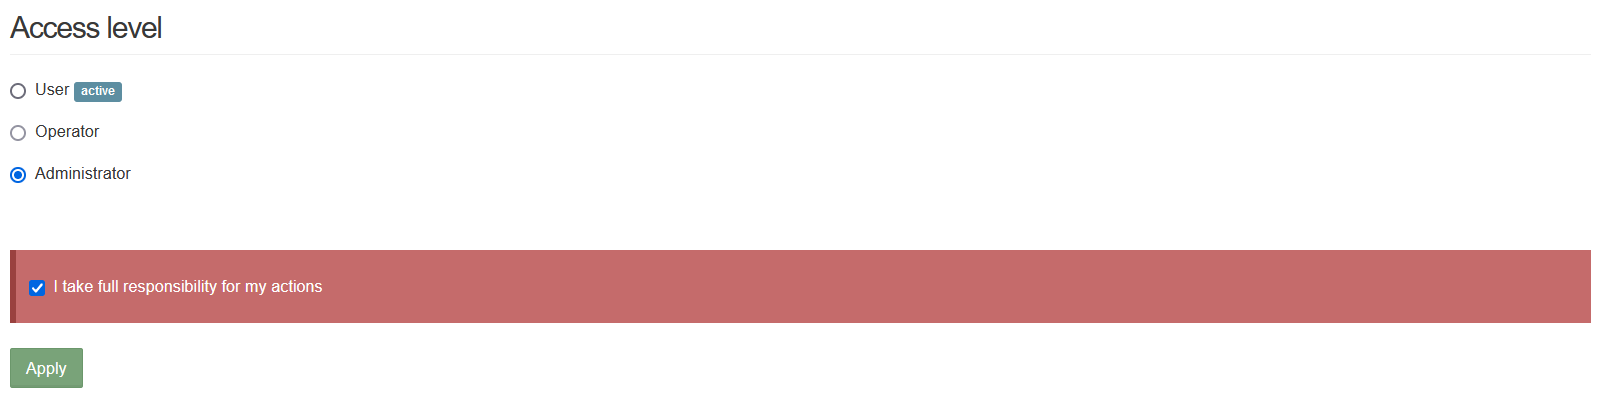
\includegraphics[width=0.6\linewidth]{images/access}
	\caption{Уровень доступа}
	\label{fig:access}
\end{figure}

\paragraph {Наличие сетевого напряжения}
Отключаем напряжение, проверяем показания датчиков энергопотребления:

% TODO: \usepackage{graphicx} required
\begin{figure}[hbpt]
	\centering
	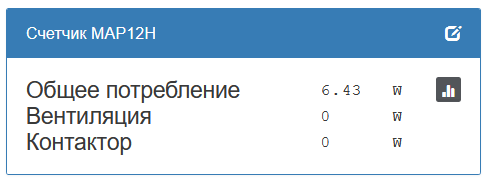
\includegraphics[width=0.5\linewidth]{images/net1}
	\caption{Наличие сетевого напряжения}
	\label{fig:net1}
\end{figure}
\newpage
% TODO: \usepackage{graphicx} required
\begin{figure}[hbpt]
	\centering
	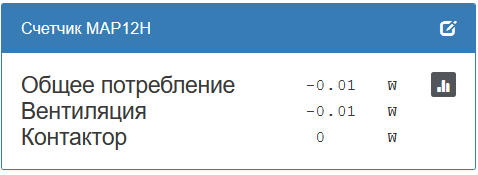
\includegraphics[width=0.5\linewidth]{images/net2}
	\caption{Изменение сетевого напряжения}
	\label{fig:net2}
\end{figure}

\paragraph{Контроль повышенного энергопотребления}
Включили вентилятор, прижали рукой, загорелся индикатор и сработала сигнализация, вентилятор выключился:
% TODO: \usepackage{graphicx} required
\begin{figure}[hbpt]
	\centering
	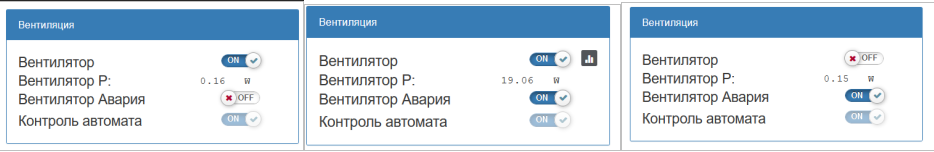
\includegraphics[width=0.6\linewidth]{images/fan-gui}
	\caption{Контроль повышенного энергопотребления}
	\label{fig:fan-gui}
\end{figure}

\paragraph{Контроль автоматов}
Отключаем питание, загораются указанные кнопки:

% TODO: \usepackage{graphicx} required
\begin{figure}[hbpt]
	\centering
	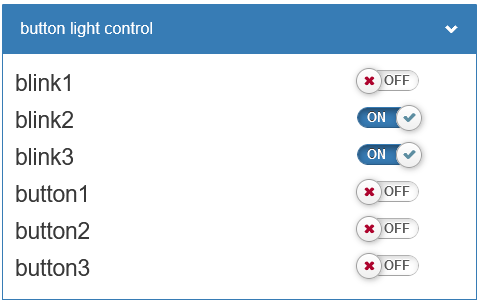
\includegraphics[width=0.5\linewidth]{images/auto-gui}
	\caption{Контроль автоматов}
	\label{fig:auto-gui}
\end{figure}
\paragraph{Контроль повышенного энергопотребления}
Включили вентилятор, прижали рукой, загорелся индикатор и сработала сигнализация, вентилятор выключился

\anonsubsection{Вывод}
В ходе данной практической работы мы выполнили настройку удаленного подключения к демонстрационному стенду  WB-demo-kit, ознакомились с веб-интерфейсом, научились снимать данные с датчиков с его помощью.
\newpage


\section{Дополнительные задания к работе №2}
После рассмотрения вышеупомянутых отраслей Интернета вещей, было принято решение разработать систему управления освещением Умного дома.

\subsection{Отраслевая принадлежность}
Данное технологическое решение относится к отрасли Умного дома, то есть находится на пользовательском уровне, но после внесения небольших изменений, может быть так же применено в промышленном секторе.
\subsection{Актуальность решения}
Актуальность данного решения обусловлена тем, что ручное управление электропитанием в жилом помещении, и освещением в частности, требует слишком большого внимания со стороны пользователя и может быть полностью автоматизировано.

При этом вероятность возникновения аварийных ситуаций снижается, а расходование ресурсов оптимизируется.

Также появляется возможность обеспечить бесперебойную работу всех потребителей питание в жилом помещении.

\subsection{Перечень оборудования}
Отладочная модель рассматриваемой системы будет построена с использованием компонентов WB-demo-kit v.2. Перечислим необходимый перечень оборудования
\begin{enumerate}
	\item Настенный комбинированный датчик WB-MSW v.3,
	\item RGB лента,
	\item Programmable Automatic Controller под управлением Debian 9.6.,
	\item Многоканальный измеритель WB-MAP12H,
	\item Автомат питания контактора,
	\item Трансформатор тока 25 А.
\end{enumerate}

\subsection{Требуемые данные} 
Для наилучшего функционирования системы необходимо располагать следующими данными о пользователях:
\begin{itemize}
	\item Период активности людей, находящихся в помещении;
	\item Степень освещенности помещения в течении дня;
	\item Уровень расхода электроэнергии;
\end{itemize}
\newpage

\section{Практическая работа №3. \\Обработка событий в системах\\Интернета вещей}

\subsection{Ход работы}

\paragraph {Задание}

Разработайте сценарии для обработки событий согласно вариантам и приведите в отчете его листинг с комментариями.

Вариант №5:
\begin{enumerate}
	\item Включение и выключение вентилятора по датчику движения.
	
	\item Включение и выключения индикации зеленым и красным светом комбинированного датчика 5 по кнопкам.
\end{enumerate}
\paragraph{Разработанные скрипты} Приведем содержание разработанных скриптов на языке JavaScript:
\setcounter{script}{0}
\script Включение и выключение вентилятора по датчику движения.
\lstinputlisting{/home/denilai/Documents/repos/latex/scripts/iot-script-1.js}
\newpage
Результат выполнения сценария:
% TODO: \usepackage{graphicx} required
\begin{figure}[htbp]
	\centering
	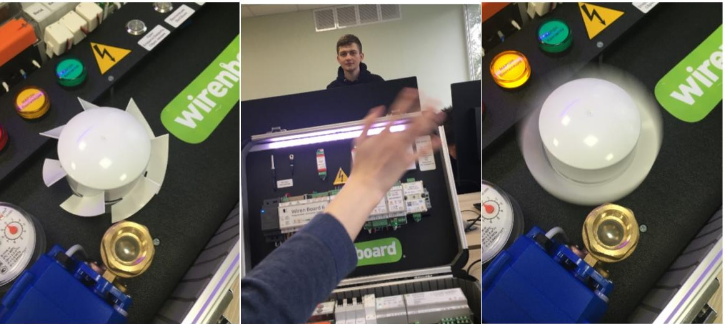
\includegraphics[width=0.7\linewidth]{images/script1-result}
	\caption{Результат 1}
	\label{fig:script1-result}
\end{figure}


\script Включение и выключения индикации зеленым и красным светом комбинированного датчика 5 по кнопка
\lstinputlisting{/home/denilai/Documents/repos/latex/scripts/iot-script-2.js}
\anonsubsection{Вывод}
В ходе данной практической работы мы получили начальные навыки написания скриптов (сценариев) для стенда WB-demo-kit  на языке JavaScript, познакомились с понятием <<правил>>, написали собственные сценарии и проверили их работоспособность на практике. 

\newpage

\section{Дополнительные задания к работе №3}
\subsection{Портрет пользователя}
Пользователем нашей системы по управлению освещением в составе инфраструктуры Умного дома может являться любой человек. Особыми техническими навыками и знаниями обладать не обязательно.

В случае, если необходимо настроить работу системы, это можно будет сделать через web интерфейс. При таком сценарии от пользователя потребуются основные навыки пользования персональным компьютером или мобильным устройством, умение взаимодействовать с графическим интерфейсом.
\subsection{Взаимодействие с системой}

При входе в помещение пользователь, двигаясь активирует датчик движения, который согласно внутренней логике устройства в зависимости от пороговых значений, а также его активности, изменяет уровень освещения или конфигурацию приборов освещения.

\subsubsection*{Ситуаций взаимодействия с сайтом}
В случае, если пользователю будет необходимо изменить конфигурацию или настройки системы освещения, ему следует посетить web-интерфейс. С помощью предоставленных инструментов пользователь сможет изменить пороговые значения или алгоритмы изменения освещения.

\subsection{Сценарии использования}
Пользователь может, находясь возле датчиков движения активировать систему, а также настроить порог активации, режимы освещения (режимы светомузыки) и цвета освещения (см. рис. \ref{fig:usecase}).

% TODO: \usepackage{graphicx} required
\begin{figure}[htbp]
	\centering
	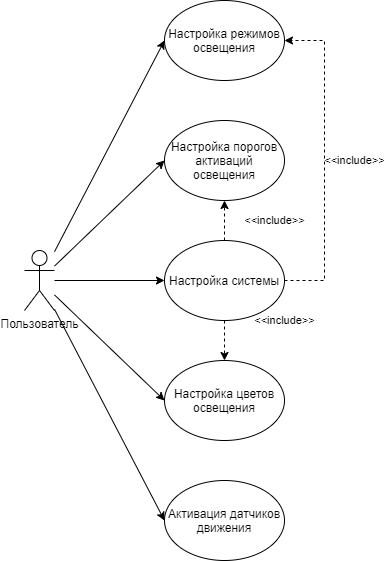
\includegraphics[width=0.5\linewidth]{images/usecase}
	\caption{Сценарии использования проекта}
	\label{fig:usecase}
\end{figure}
\newpage


\section{Практическая работа №4. \\Основы электротехники в системах\\Интернета вещей}
\subsection{Ход работы}
\paragraph{Описание сценариев} Приведем sequence диаграмму, построенные на основании первого сценария, описанного выше.
% TODO: \usepackage{graphicx} required
\begin{figure}[htbp]
	\centering
	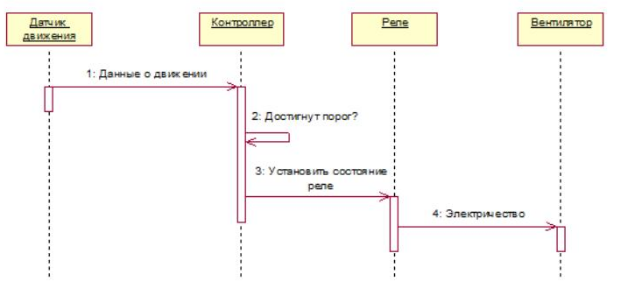
\includegraphics[width=0.7\linewidth]{images/deploy-scheme}
	\caption{Sequence диаграмма по первому сценарию}
	\label{fig:deploy-scheme}
\end{figure}

Приведем схему подключения элементов, необходимых для реализации первого сценария.
% TODO: \usepackage{graphicx} required
\begin{figure}[htbp]
	\centering
	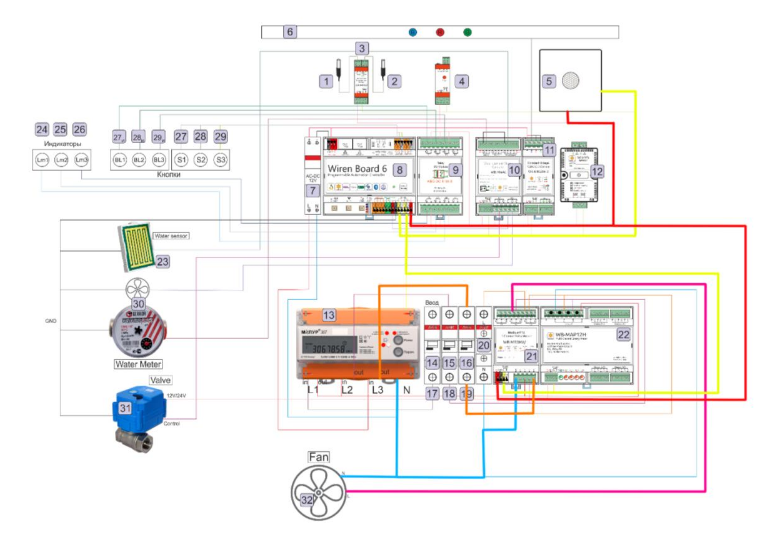
\includegraphics[width=0.7\linewidth]{images/deploy-scheme-demo}
	\caption{Схема подключения по первому сценарию}
	\label{fig:deploy-scheme-demo}
\end{figure}
Приведем sequence диаграмму, построенные на основании второго сценария, описанного выше.
% TODO: \usepackage{graphicx} required
\begin{figure}[htbp]
	\centering
	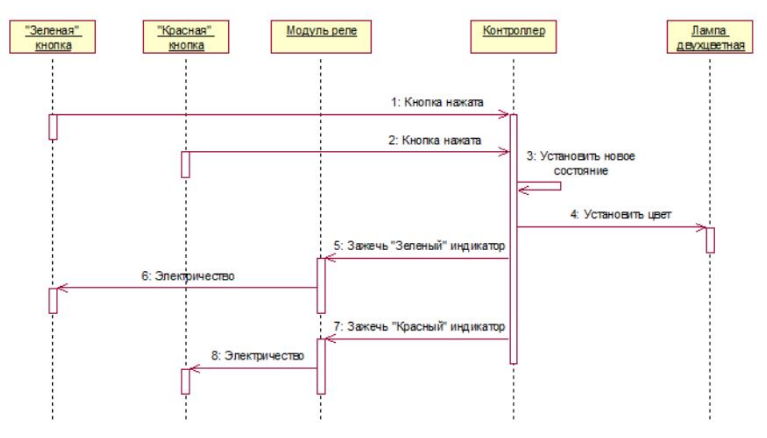
\includegraphics[width=0.7\linewidth]{images/deploy-scheme2}
	\caption{Sequence диаграмма по второму сценарию}
	\label{fig:deploy-scheme2}
\end{figure}
Приведем схему подключения элементов, необходимых для реализации второго сценария.
% TODO: \usepackage{graphicx} required
\begin{figure}[htbp]
	\centering
	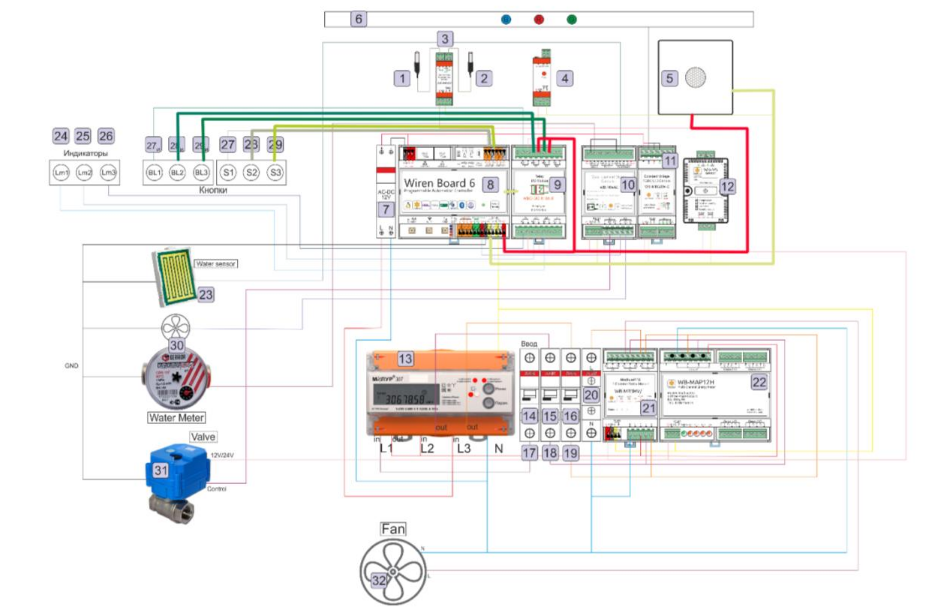
\includegraphics[width=0.7\linewidth]{images/deploy-scheme-demo2}
	\caption{Схема подключения по второму сценарию}
	\label{fig:deploy-scheme-demo2}
\end{figure}
\anonsubsection{Вывод}
В ходе данной практической работы мы описали созданные сценарии в методологии UML с помощью sequence диаграмм, продумали схему подключения модулей и компонентов, необходимых для их реализации.

\newpage
\section{Дополнительные задания к работе №4}
\subsection{Требования к проекту}
\begin{enumerate}
	\item Отказоустойчивость. Организовать бесперебойную работу сайта (приложения), в случае возникновения ошибок предоставить отчет.
	
	\item Простота эксплуатации. Система должна предоставлять удобный интерфейс для настройки и взаимодействия аппаратных элементов.
	
	\item Возможность повторного использования. Необходимо предусмотреть возможность расширения функционала предложения.
	
	\item Проект должен быть построен на базе демонстрационного стенда WB-demo-kit v.2. Взаимодействие датчиков и пользователя должно быть реализовано через веб-ресурс.
\end{enumerate}
\subsection{Требования к данным}
\begin{enumerate}
	\item 
\end{enumerate}
\subsection{Архитектура проекта}
\begin{itemize}
	\item Проект выполнен на базе демонстрационного стенда WB-demo-kit v.2.
	
	\item Сайт поддерживается через WB-demo-kit v.2 на основе Nginx.
	
	\item Все датчики связаны между собой посредством внутренней логики WB-demo-kit v.2.
	
	\item Описание поведения светодиодной ленты осуществляется с помощью языка JavaScript.
	\item Передача данных осуществляется с использованием стандартов ZigBee и Bluetooth и протоколов стека TCP/IP. 
	
\end{itemize}

Приведем архитектуры проекта в виде схемы (см. рис. \ref{fig:architecture}).
% TODO: \usepackage{graphicx} required
\begin{figure}[htbp]
	\centering
	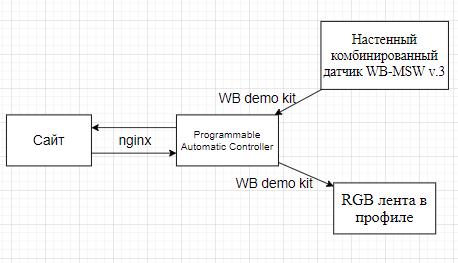
\includegraphics[width=0.5\linewidth]{images/architecture}
	\caption{Архитектура системы}
	\label{fig:architecture}
\end{figure}
\newpage
\subsection{Оборудование для реализации проекта}
\begin{itemize}
	\item WB-demo-kit v.2:
	\begin{enumerate}
		\item Настенный комбинированный датчик WB-MSW v.3,
		\item RGB лента,
		\item Programmable Automatic Controller под управлением Debian 9.6.,
		\item Многоканальный измеритель WB-MAP12H,
		\item Автомат питания контактора,
		\item Трансформатор тока 25 А.
	\end{enumerate}
	\if 0
	\item Минимальные требования к личному ПК:
	\begin{enumerate}
		\item OS: Windows ХР/Linux,
		\item Процессор: Intel Celeron или аналоги,
		\item Доступ в Интернет 128 Кбит/c.
	\end{enumerate}
	\fi
\end{itemize}
\end{document}


